\documentclass[letter, 11pt]{article}
\usepackage[utf8]{inputenc}
\usepackage[spanish]{babel}
\usepackage{amsfonts}
\usepackage[dvips]{graphicx}
\usepackage{url}
\usepackage{graphicx} %Permite exportar imagenes en formato eps
\usepackage{url} %Tipo de fuente para correos y paginas
\usepackage{pgf}
\usepackage{fleqn}
\usepackage{amssymb}
\usepackage{amsmath}
\usepackage{fancyvrb}
\usepackage{makeidx}
\usepackage{colortbl} %Permite colocar colores a las tablas
\usepackage{multirow}
\usepackage{booktabs}
\usepackage{moreverb}
\usepackage{rotating}
\usepackage[final]{pdfpages}

%\usepackage[top=3cm,bottom=3cm,left=3.5cm,right=3.5cm,footskip=1.5cm,headheight=1.5cm,headsep=.5cm,textheight=3cm]{geometry}

%%%%%%%%%%
%Margenes%
%%%%%%%%%%
\parskip 1mm %Espacio entre parrafos

\setlength{\topmargin}{0pt}
\topmargin      0.5cm
\oddsidemargin	0.1cm  % Ancho Letter 21,59cm
\evensidemargin 0.5cm  % Alto  Letter 27,81cm
\textwidth	14cm
\textheight	21.0cm
\headsep	4 mm
\parindent	0.5cm


\begin{document}
\title{Inteligencia Artificial \\ \begin{Large}Estado del Arte: Problema \textit{Aircraft Landing Scheduling}\end{Large}}
\author{Victor Gonzalez Rodriguez\\ \url{victor.gonzalezro@alumnos.usm.cl}}
\date{\today}
\maketitle


%--------------------No borrar esta secci\'on--------------------------------%
\section*{Evaluación}

\begin{tabular}{ll}
Resumen (5\%): & \underline{\hspace{2cm}} \\
Introducci\'on (5\%):  & \underline{\hspace{2cm}} \\
Definici\'on del Problema (10\%):  & \underline{\hspace{2cm}} \\
Estado del Arte (35\%):  & \underline{\hspace{2cm}} \\
Modelo Matem\'atico (20\%): &  \underline{\hspace{2cm}}\\
Conclusiones (20\%): &  \underline{\hspace{2cm}}\\
Bibliograf\'ia (5\%): & \underline{\hspace{2cm}}\\
 &  \\
\textbf{Nota Final (100\%)}:   & \underline{\hspace{2cm}}
\end{tabular}
%---------------------------------------------------------------------------%
\vspace{2cm}


\begin{abstract}
En este informe, consideramos el problema de Aircraft Landing Scheduling, donde se modela el aterrizaje de aviones en distintas pistas de un aeropuerto. Este problema nos ayuda a decidir el tiempo y lugar donde un avión debería aterrizar dentro de una ventana predeterminada de tiempo, respetando la separación de tiempo entre aterrizajes y la secuencia respectiva de aviones que deben aterrizar después. Analizaremos el estado del arte de los métodos actualmente publicados, de manera que se genere una idea general de las implementaciones disponibles para resolver este problema, y analizar así cuales son los mejores acercamientos y sus evoluciones. Finalmente, esto se presentará mediante un modelo matemático, formulando sus respectivas restricciones y variables, para luego comentar y concluir el estado del arte al presente año.
\end{abstract}

\begin{description}
\item[Keywords:] Aircraft Landing Scheduling problem, estado del arte, modelo matemático, calendarización de aterrizajes, Aircraft Arrival and Departure Sequencing problem.
\end{description}
\newpage

\section{Introducción}
El Aircraft Landing Scheduling Problem (ALSP), o \textit{Problema de Calendarización de Aterrizaje de Aeronaves} en español, es un problema que ha ganado mucha importancia a nivel mundial, especialmente los últimos años debido a la gran congestión de aviones que están circulando actualmente en el espacio aéreo mundial, y la necesidad de mantener el flujo de aeronaves lo más fluido posible sin perder de vista la seguridad de los pasajeros que son parte escencial de todo este sistema. Ejemplo de esto es la investigación impulsada gubernamentalmente en el aeropuerto de Heathrow hace un par de años atrás.

El ALSP es catalogado como un problema muy complejo, el cual en la clasificación estándar, se lo cataloga como NP-complejo\footnote{Tan complejo como el más dificil de los problemas polinomiales no-deterministas.}, y debido a esto mismo, las implementaciónes disponibles en las publicaciones a nivel mundial, pueden llegar a ser muy complejas y difíciles de entender. Debido a esta situación, hemos de entregar una definición del problema que sólo involucre los factores más comunes y/o significativos para modelar el ALSP, y a partir de esto, se presentará un modelo matemático tan sencillo como la definición del problema lo permita.

Estudiaremos ademas, las distintas implementaciones disponibles actualmente de manera superficial, de modo que se pueda comparar a grandes rasgos cual es la tendencia mundial o histórica para resolver este tipo de problemas, situando al lector en la situación actual de la modelación de estos problemas.

A partir de lo presentado previamente en este documento, se comentará, justificará y comentará lo expuesto en la sección llamada \textit{Estado del Arte} y \textit{Modelo Matemático}.

Finalmente, es de esperar que la información entregada en este documento, sea de ayuda para tener una buena noción de lo que está ocurriendo actualmente respecto al ALSP, y cuales serían los mejores acercamientos para resolver este tipo de problemas en la actualidad.

\section{Definición del Problema}
Debido a la creciente demanda de vuelos al rededor del mundo durante las últimas décadas, junto con el impulso de la tecnología y el explosivo aumento de pasajeros, ha puesto a los aeropuertos manejando cientos viajes en un día. Todo esto sin dejar de lado la seguridad, los tiempos de despegue/aterrizaje y la optimización del uso de los recursos de infraestructura.

Para darnos una idea gráfica del tráfico actual en el mundo, disponemos de la siguiente captura del día viernes 10 de mayo de 2013 a las 19:00 horas aproximadamente.
\begin{figure}[!h]
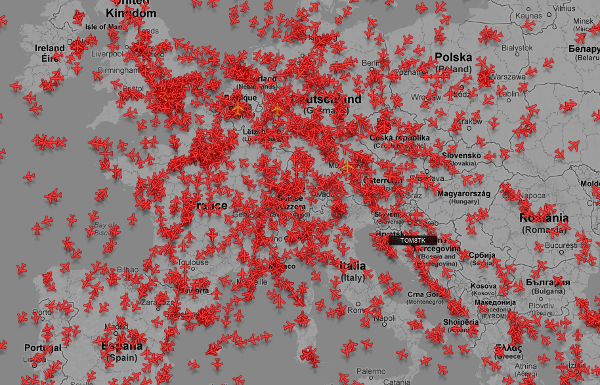
\includegraphics[width=13.5cm]{aviones.png}
\centering
\caption{Fuente: http://www.planefinder.net/}
\end{figure}

\section{Estado del Arte}
Lo m\'as importante que se ha hecho hasta ahora con relaci\'on al problema. Deber\'ia responder preguntas como las siguientes:
?`cuando surge?, ?`qu\'e m\'etodos se han usado para resolverlo?, ?`cuales son los mejores algoritmos que se han creado hasta
la fecha?, ?`qu\'e representaciones han tenido los mejores resultados?, ?`cu\'al es la tendencia actual?, tipos de movimientos,
heur\'isticas, m\'etodos completos, tendencias, etc... Puede incluir gr\'aficos comparativos, o explicativos.\\
La informaci\'on que describen en este punto se basa en los estudios realizados con antelaci\'on respecto al tema.
Dichos estudios se citan de manera que quien lea su estudio pueda tambi\'en
 acceder a las referencias que usted revis\'o. Las citas se realizan mediante el comando \verb+\cite{ }+.
Por ejemplo, para hacer referencia al art\'iculo de algoritmos h\'ibridos para problemas de satisfacci\'on 
 de restricciones que ley\'o para el primer certamen~\cite{Prosser93Hybrid}.

\section{Modelo Matem\'atico}
Uno o m\'as modelos matem\'aticos para el problema, idealmente indicando el espacio de b\'usqueda para cada uno.

\section{Conclusiones}
Conclusiones RELEVANTES del estudio realizado.

\section{Bibliograf\'ia}
Indicando toda la informaci\'on necesaria de acuerdo al tipo de documento revisado. Todas las referencias deben ser 
citadas en el documento.
\bibliographystyle{plain}
\bibliography{Referencias}

\end{document} 
